\section{Factory Spiel in Unity}\label{sec:factory}
Um zu sehen, welches Potential die datenorientierte Programmierung in der Spieleentwicklung bietet wurde eine Spielsimulation sowohl datenorientiert als auch objektorientiert erstellt. Das Spiel, welches simuliert und gemessen wird ist eine Art Aufbauspiel. Verglichen kann es mit dem populären Spiel Factorio\footnote{https://www.factorio.com/}. Hier wird es jedoch etwas schlichter und einfacher gehalten. Um beide Programmierparadigmen miteinander zu vergleichen wird eine kleine Fabrik in die Spielwelt generiert und vervielfältigt. Dies soll den Spieler simulieren. In Abbildung \ref{fig:steel} sieht man wie eine Produktionsstraße für Stahl in dem Spiel aussehen kann:
\begin{figure}[H]
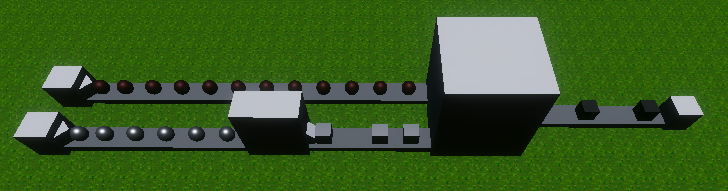
\includegraphics[scale=0.87]{Bilder/Stahl Fabrik.png}
\caption{Eine Stahl Fabrik in der Unity Spielesimulation.}
\label{fig:steel}
\end{figure}
Ganz links befinden sich zwei Kästen. Diese sollen Erzbohrer darstellen welche Eisenerz (silbern) und Kohle (braun) aus der Erde befördern und rechts auf ein Förderband legen. Die beiden Förderbänder transportieren die Kohle und das Eisenerz nach rechts weiter. Das Eisenerz wird als nächstes in Eisenbarren geschmolzen und sind deshalb rechteckig. Die Kohle und die Eisenbarren kommen dann gemeinsam in den großen Würfel, wo sie zu Stahl verarbeitet werden. Dieser Stahl wird dann wieder auf ein Förderband gelegt und in dem kleinen Würfel anschließend gelöscht. Die ganze Produktionskette soll möglichst einem Spiel nahekommen damit es eine möglichst realistische Simulation bietet und die Realität widerspiegelt. Nachfolgend wird gezeigt, wie die Spielsimulation möglichst ähnlich umgesetzt und gebenchmarkt wird.
\subsection{Objektorientierte Programmierung}
In der Objektorientierten Programmierung mit Unity dreht sich alles um GameObjects. Jedes Objekt in der Szene, egal ob sichtbar oder nicht ist ein GameObject. Diese GameObjects können verschiedene Komponenten haben, welche Eigenschaften definieren, also Daten speichern. Diese Komponenten sind jedoch nicht zu verwechseln mit den \textit{Components} aus dem datenorientierten Ansatz von Unity. Diese Komponenten haben jeweils eine \texttt{Start} und eine \texttt{Update} Methode welche das Verhalten definieren. Die Start Methode wird einmalig vor dem ersten Aufruf der \texttt{Update} Methode ausgeführt. Die \texttt{Update} Methode läuft ein mal pro ausgegebenem Bild. Das Skript für das Item sieht wie folgt aus:
\begin{lstlisting}[style=code, caption={Item Komponente OOP}]
using Unity.Mathematics;
using UnityEngine;

public class Item : MonoBehaviour
{
    private int2 pos;
    //Serialisiertes Feld für den Unity Editor
    [SerializeField] private int itemID;

    void Update()
    {
    	//Gegenstand wird zu der übergebenen Position pos bewegt
        transform.position = Vector3.Lerp(transform.position, new Vector3(pos.x, pos.y, -0.5f), Time.deltaTime * 2f);
    }

    public void SetPosition(int2 pos)
    {
        this.pos = pos;
    }

    public int GetItemID()
    {
        return itemID;
    }
}
\end{lstlisting}
Wie man sieht beinhaltet das MonoBehaviour nicht nur die Daten, sondern auch die Logik. Für ein Item benötigen wir zum einen die Position, wohin sich das Item bewegen soll, zum anderen speichern wir auch eine ID über die wir das Item ganz einfach identifizieren können. Das Attribut \glqq SerializeField\grqq{} zwingt Unity dazu ein editierbares Feld im Editor zu erstellen an dem man die itemID setzen kann.
\begin{figure}[H]
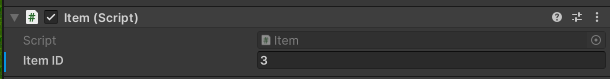
\includegraphics[scale=1]{Bilder/SerializeField.png}
\caption{Ein editierbares Feld in dem Unity Editor. Das Feld wird durch ein public Attribut, oder dem SerializeField Flag erzeugt.}
\label{fig:SerializeField}
\end{figure}
Eine Start Funktion ist in diesem Fall nicht notwendig. Die \texttt{Update} Methode bewegt das Item langsam an die übergebene Position. Time.deltaTime gibt die Zeit in Sekunden von dem letzten Bild bis zu dem momentanen Bild an. Dadurch wird die Bewegung linear.\\Ein weiterer Teil der Simulation ist die Bewegung der Items über das Förderband: 
\begin{lstlisting}[style=code, caption={Förderband Komponente OOP}]
using System.Collections.Generic;
using UnityEngine;

namespace Buildings.Components
{
    public class BeltPath : MonoBehaviour
    {
        private List<ConveyorComponent> beltPath = new ();
        private InputConveyorComponent input;
        private OutputConveyorComponent output;
        private float timeToMove;

        public void Start()
        {
        	//Referenzen auf die Komponenten des GameObjects werden geholt
            input = GetComponent<InputConveyorComponent>();
            output = GetComponent<OutputConveyorComponent>();
            timeToMove = 2f;
        }

        public void Update()
        {
            timeToMove -= Time.deltaTime;
            if(timeToMove > 0) return;
            
            //Gegenstände nach 2 Sekunden bewegen
            var lastBelt = beltPath[^1];
            if (!ReferenceEquals(lastBelt.item, null) && ReferenceEquals(output.GetItem(), null))
            {
            	//Gegenstand von dem letzten Förderbandsegment auf den Output legen
                var item = lastBelt.item;
                var itemComponent = item.GetComponent<Item>();
                itemComponent.SetPosition(output.GetPosition());
                output.SetItem(item);
                lastBelt.item = null;
            }
            //Gegenstände von hinten nach vorne verschieben
            for (int i = beltPath.Count-2; i >= 0; i--)
            {
                var thisConveyor = beltPath[i];
                var lastConveyor = beltPath[i + 1];
                if (!ReferenceEquals(thisConveyor.item, null))
                {
                    if (ReferenceEquals(lastConveyor.item, null))
                    {
                        var item = thisConveyor.item;
                        var itemComponent = item.GetComponent<Item>();
                        lastConveyor.item = item;
                        //Position des Gegenstandes aktualisieren
                        itemComponent.SetPosition(lastConveyor.pos);
                        thisConveyor.item = null;
                    }
                }
            }
            var firstConveyor = beltPath[0];
            //TODO eventuell noch besser machen
            if (!ReferenceEquals(firstConveyor.item, null)) input.SetOccupied(true);
            else input.SetOccupied(false);
            if (!ReferenceEquals(input.GetItem(), null) && ReferenceEquals(firstConveyor.item, null))
            {
                firstConveyor.item = input.GetItem();
                input.RemoveItem();
            }
            timeToMove += 2f;
        }

        public void AddConveyor(ConveyorComponent conveyorComponent)
        {
            beltPath.Add(conveyorComponent);
        }
    }
}
\end{lstlisting}
Für das Förderband wird eine Liste mit vorhandenen Segmenten, der Input, der Output und eine Zeit gespeichert. Die Zeit wird in der Start Methode initialisiert und der Input bzw. Output wird über die Funktion \glqq GetComponent()\grqq{} von dem GameObject geholt. In der \texttt{Update} Funktion wird zunächst nur die timeToMove Variable herunter gezählt. Sollte diese Variable unter Null fallen, werden alle Items von hinten nach vorne ein Segment weiter bewegt sofern dies möglich ist. Ist der Output nicht belegt wird ein vorhandenes Item in den Output gelegt. Items auf den einzelnen Segmenten werden nach weiterbewegt und wenn ein Item im Input liegt wird dies auf das erste Segment weiterbewegt. Immer wenn ein Item weitergegeben wird (egal ob an ein Segment, oder an den Output) wird auch die neue Position an das Item weitergegeben. Durch das bewegen der Items von hinten nach vorne verhindert man, dass sich Items nicht bewegen, obwohl sie es könnten.
\subsection{Datenorientierte Programmierung}
In der datenorientierten Programmierung gehen wir statt der GameObjects auf die Komponenten und Systeme ein. Auch hier zu Beginn die Komponente für ein Item und das dazugehörige System:
\begin{lstlisting}[style=code, caption={Item Komponente ECS}]
using Unity.Entities;
using Unity.Mathematics;

namespace ECS.Components
{
    public struct ItemComponent : IComponentData
    {
        public int2 pos;
        public int itemID;
    }
}
\end{lstlisting}
Auch hier wird die Position und die ID des Items gespeichert. Das dazugehörige System sieht anders aus als das MonoBehaviour im Objektorientierten, die Logik ist jedoch dieselbe:
\begin{lstlisting}[style=code, caption={Item System}]
using ECS.Components;
using Unity.Burst;
using UnityEngine;
using Unity.Entities;
using Unity.Transforms;

[BurstCompile(CompileSynchronously = true)]
public partial struct ItemSystem : ISystem
{
    
    [BurstCompile(CompileSynchronously = true)]
    public void OnUpdate(ref SystemState state)
    {
    	//Job erstellen, Zeit übergeben und schedulen
        new ItemMoveJob
        {
            deltaTime = SystemAPI.Time.DeltaTime
        }.ScheduleParallel();
    }

    [BurstCompile(CompileSynchronously = true)]
    public partial struct ItemMoveJob : IJobEntity
    {
        public float deltaTime;
        
        [BurstCompile(CompileSynchronously = true)]
        private void Execute(ref LocalTransform transform, in ItemComponent item)
        {
        	//Gegenstand wird zu der übergebenen Position pos bewegt
            transform = transform.WithPosition(Vector3.Lerp(transform.Position.xyz, new Vector3(item.pos.x, item.pos.y, -0.5f), deltaTime * 2f));
        }
    }
}
\end{lstlisting}
Jedoch sieht man hier schon Eigenheiten des Entity Component Systems, des Burst Compiler und dem Job System. Das Item System implementiert das Interface ISystem welches für unverwaltete Systeme verwendet werden muss. Zusätzlich ist die Struktur als auch deren Methoden und dem Job mit BurstCompile gekennzeichnet. Diese Kennzeichnung hilft dem Burst Compiler Methoden zu finden, welche mit Burst kompiliert werden sollen. Das Flag CompileSynchronously dient dem testen. Es besagt, dass erst das System durch den Burst Compiler kompiliert werden muss bevor es laufen kann. Andernfalls könnte das System schon laufen, ohne den Burst Compiler genutzt zu haben. Die Methode \texttt{OnUpdate} wird ein mal pro Bild aufgerufen. Sie ist zu vergleichen mit der \texttt{Update} Methode in einem MonoBehaviour. Innerhalb der \texttt{OnUpdate} Methode kommt das Job System von Unity zum Einsatz. Es wird der ItemMoveJob erstellt. Dieser Job funktioniert mit einem LocalTransform Component, welches jedes Entity besitzt und mit dem ItemComponent. Dabei wird das LocalTransform Component zum lesen und schreiben verwendet (erkennbar durch das Keywort ref) und das ItemComponent lediglich zum lesen (erkannbar durch das Keywort in). Auch hier wird nun die Position des Items mithilfe der Lerp Funktion von Vector3 und den Daten im ItemComponent verändert. Dieser Job, welcher die tatsächliche Logik für das Item enthält wird in der \texttt{OnUpdate} Methode parallel gescheduled. Dies ist hier speziell sehr vorteilhaft, da es sehr viele Items auf dem Spielfeld geben kann. Dadurch werden nicht tausende Items nacheinander bewegt, sondern alle zur gleichen Zeit.\\Ein Blick sollte auch auf das Erstellen und Zerstören von Items gelegt werden:
\begin{lstlisting}[style=code, caption={Create Item System}]
using ECS.Components;
using ECS.Components.Other;
using Unity.Burst;
using Unity.Collections;
using Unity.Entities;
using Unity.Mathematics;
using Unity.Transforms;
using UnityEngine;

namespace ECS.Systems
{
    [BurstCompile(CompileSynchronously = true)]
    [UpdateAfter(typeof(ProcessingBuildingSystem))]
    public partial struct CreateItemSystem : ISystem
    {
        private ComponentLookup<InputConveyorComponent> inputLookup;

        [BurstCompile(CompileSynchronously = true)]
        public void OnCreate(ref SystemState state)
        {
        	//Für die OnUpdate Funktion wird das ItemEntitiesComponent gebraucht
            state.RequireForUpdate<ItemEntitiesComponent>();
            inputLookup = state.GetComponentLookup<InputConveyorComponent>();
        }

        [BurstCompile(CompileSynchronously = true)]
        public void OnUpdate(ref SystemState state)
        {
            inputLookup.Update(ref state);
            var ecbSingleton = SystemAPI.GetSingleton<BeginSimulationEntityCommandBufferSystem.Singleton>();
            //Entity Command Buffer wird erstellt
            var ecb = ecbSingleton.CreateCommandBuffer(state.WorldUnmanaged);
            var itemEntities = SystemAPI.GetSingleton<ItemEntitiesComponent>();
            new CreateItemJob
            {
                inputLookup = inputLookup,
                ecb = ecb,
                itemEntities = itemEntities
            }.Schedule();
            state.CompleteDependency();
        }
        
        [BurstCompile(CompileSynchronously = true)]
        [WithNone(typeof(OutputNotFoundTag))]
        public partial struct CreateItemJob : IJobEntity
        {
            public EntityCommandBuffer ecb;
            [ReadOnly] public ComponentLookup<InputConveyorComponent> inputLookup;
            [ReadOnly] public ItemEntitiesComponent itemEntities;

            [BurstCompile(CompileSynchronously = true)]
            private void Execute(ref OutputProcessingBuildingComponent output)
            {
                if(output.itemID == -1) return;
                var itemID = output.itemID;
                var input = inputLookup[output.outputEntity];
                if(input.occupied || input.item != Entity.Null) return;
                output.itemID = -1;
                output.itemCreated = true;
                var itemEntity = itemEntities.GetEntityWithID(itemID);
                var item = ecb.Instantiate(itemEntity);
                ecb.SetComponent(item, LocalTransform.FromPositionRotationScale(new float3(output.pos.x, output.pos.y, -0.5f), quaternion.identity, 0.5f));
                ecb.SetComponent(item, new ItemComponent{pos = output.pos, itemID = itemID});
                ecb.SetComponent(output.outputEntity, new InputConveyorComponent{ item = item, pos = input.pos, occupied = true});
            }
        }
    }
}
\end{lstlisting}
Auch hier sieht man eine Besonderheit des \textit{Entity Component Systems}, der \textit{Entity Command Buffer} (ECB). Dadurch dass strukturelle Änderungen nur auf dem Haupt \textit{Thread} passieren dürfen braucht man einen ECB um diese Änderungen zu sammeln und an späteren Stelle auf dem Haupt \textit{Thread} auszuführem\footnote{https://docs.unity3d.com/Packages/com.unity.entities@1.0/manual/systems-entity-command-buffers.html}. Hier wird der ECB verwendet um strukturelle Änderungen aus einem Job vorzunehmen. Der \textit{Entity Command Buffer} erstellt das Item und ändert noch in den Komponenten die Position des Items.